% !TeX root = Main.tex

\chapter{Odvození vlnových rovnic} \label{kap:Odvozeni_VlnR}
\section{Obecně časově proměnné pole} \label{sec:Odvozeni_CasPole}
K~sestavení vlnové diferenciální rovnice pro vektor intenzity elektrického pole $\vec E$ nebo vektor indukce magnetického pole $\vec B$ využijeme diferenciální tvar Maxwellových rovnic. 
\subsection*{Maxwellovy rovnice v~diferenciálním tvaru}
\begin{equation}
	\rot\vec H = \vec J+\frac{\partial\vec D}{\partial t},
	\label{rce:1MaxwR}
\end{equation}
\begin{equation}
	\rot\vec E = -\frac{\partial\vec B}{\partial t},
	\label{rce:2MaxwR}
\end{equation}
\begin{equation}
	\div\vec D = \rho,
	\label{rce:3MaxwR}
\end{equation}
\begin{equation}
	\div\vec B = 0.
	\label{rce:4MaxwR}
\end{equation}

\subsection{Vlnová rovnice pro vektor intenzity elektrického pole $\vec E$}
Dle \cite[str. 33]{emp} uvažujeme případ, že se v~daném objemu nachází indukovaný proud a~navíc proud, který vnucen vnějším zdrojem. Důsledkem je modifikace rovnice (\ref{rce:1MaxwR})
\begin{equation}
	\rot\vec H = \vec J+\frac{\partial\vec D}{\partial t}+\vec J_{\mathrm{ext}}.
	\label{rce:1MaxwR_vn}
\end{equation}
\begin{figure}[!h]
	\centering
	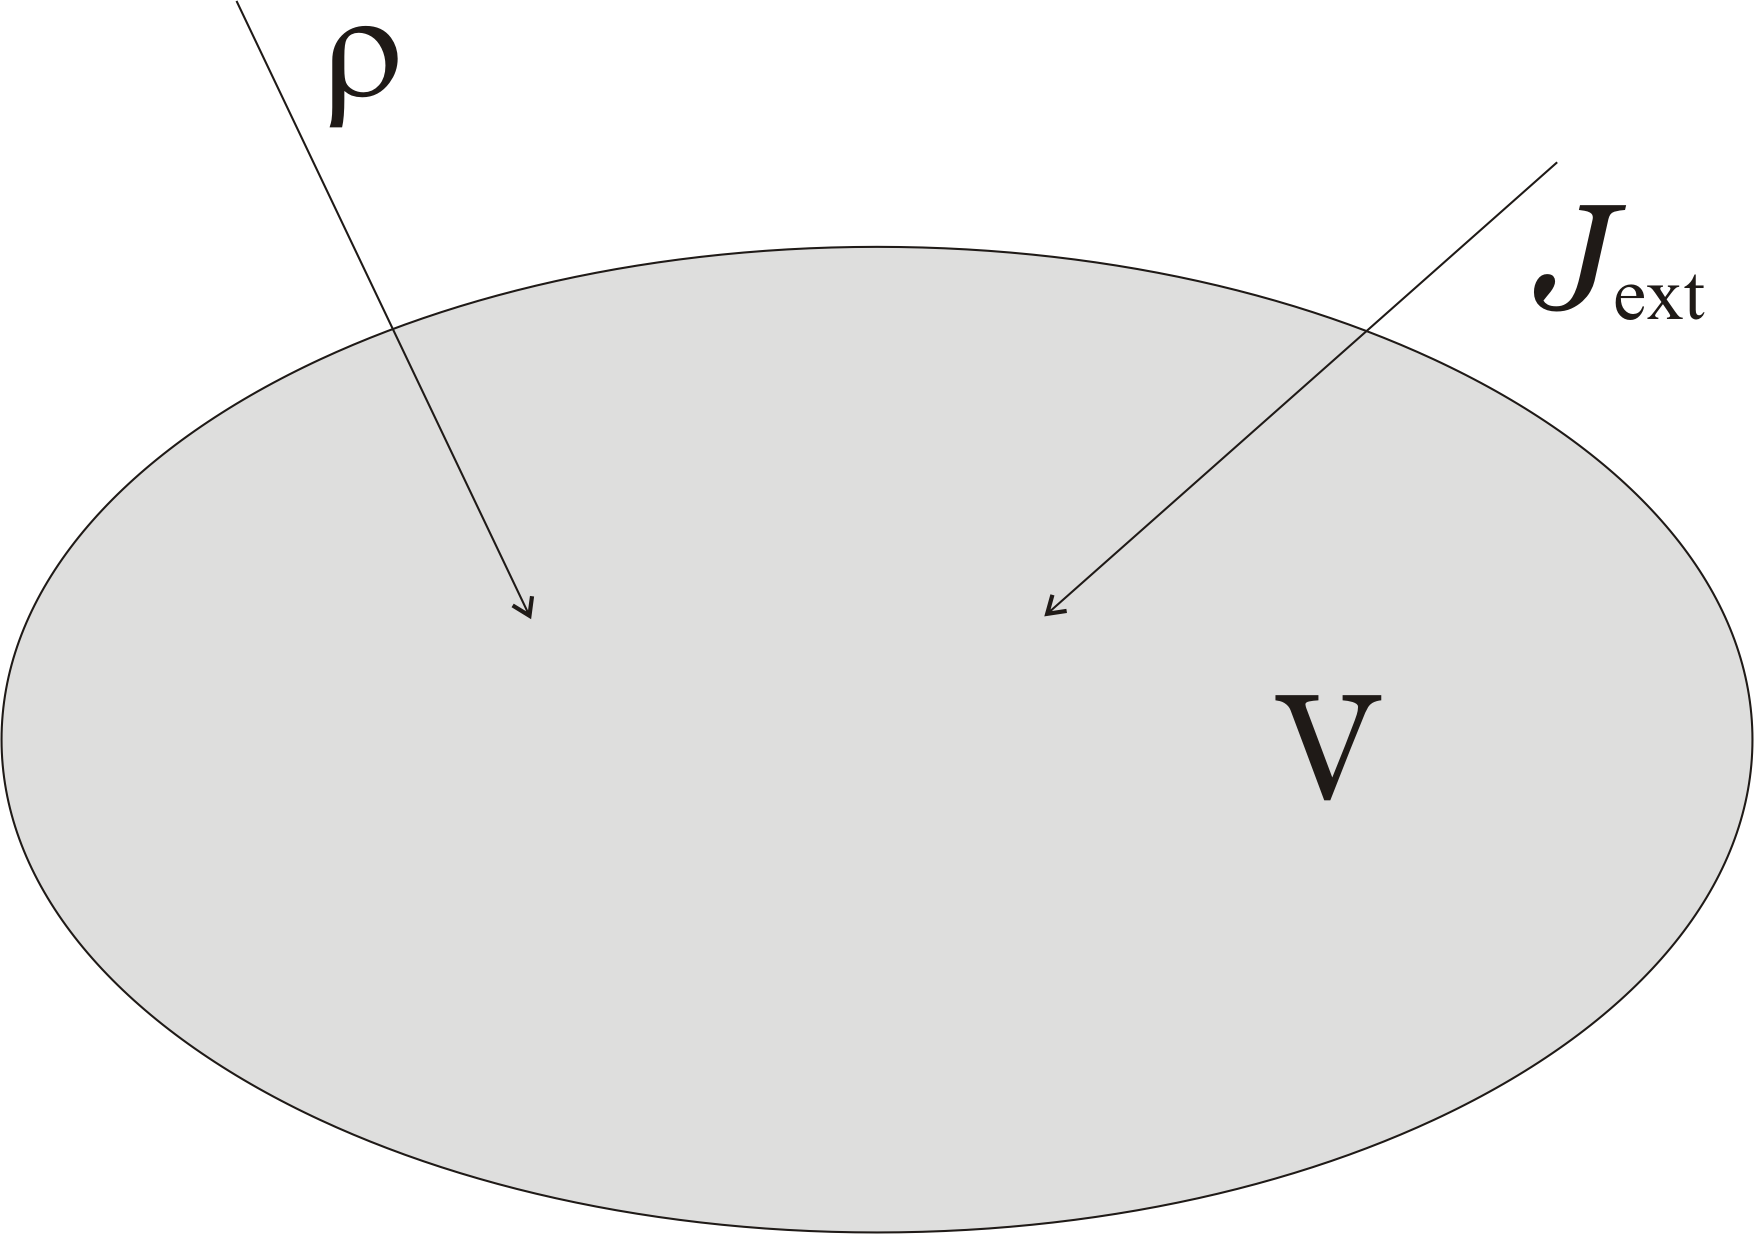
\includegraphics[width=4.5cm]{vnuceny_I.png}
	\caption{Vnucený proud vnějším zdrojem.}
	\label{obr:vnuceny_I}
\end{figure}\\
Vyjádření $\rot\vec B$ z~rovnice (\ref{rce:1MaxwR_vn})
\begin{displaymath}
	\frac{1}{\mu} \rot\vec B = \sigma \vec E+\varepsilon\frac{\partial\vec E}{\partial t}+\vec J_{\mathrm{ext}},
\end{displaymath}
\begin{equation}
	\rot\vec B = \mu\sigma\vec E+\mu\varepsilon\frac{\partial\vec E}{\partial t}+\mu\vec J_{\mathrm{ext}}.
	\label{rce:VlnR_ElPole_odv1}
\end{equation}
Na druhou Maxwelovu rovnici (\ref{rce:2MaxwR}) aplikujeme operaci rotace
\begin{displaymath}
	\rot\rot\vec E = -\frac{\partial}{\partial t}\rot\vec B.
\end{displaymath}
Za výraz $\rot\vec B$ na pravé straně rovnice dosadíme z~(\ref{rce:VlnR_ElPole_odv1})
\begin{displaymath}
	\rot\rot\vec E = -\frac{\partial}{\partial t}\Big(\mu\sigma\vec E+\mu\varepsilon\frac{\partial\vec E}{\partial t}+\mu\vec J_{\mathrm{ext}}\Big).
\end{displaymath}
Pravou stranu rovnice roznásobíme a na levou použijeme vztah vektorové identity $\rot\rot\vec E = \grad\div\vec E - \nabla^{2}\vec E$ 
\begin{displaymath}
	\grad\div\vec E - \nabla^{2}\vec E = -\mu\sigma\frac{\partial\vec E}{\partial t}-\mu\varepsilon\frac{\partial^{2}\vec E}{\partial t^{2}}-\mu\frac{\partial\vec J_{\mathrm{ext}}}{\partial t}.
\end{displaymath}
Ze třetí Maxwellovy rovnice (\ref{rce:3MaxwR}) dosadíme za $\div\vec E$ výraz $\frac{\rho}{\varepsilon}$. Úpravou přesuneme na~pravou stranu zdrojové funkce elektromagnetického pole a dostaneme výslednou vlnovou rovnici pro vektor intenzity elektrického pole $\vec E$
\begin{equation}
	\nabla^{2}\vec E -\mu\sigma\frac{\partial\vec E}{\partial t}-\mu\varepsilon\frac{\partial^{2}\vec E}{\partial t^{2}} = \grad\frac{\rho}{\varepsilon}+\mu\frac{\partial\vec J_{\mathrm{ext}}}{\partial t}.
	\label{rce:VlnR_ElPole}
\end{equation}
Rovnice (\ref{rce:VlnR_ElPole}) je dle \cite{emp} označována jako {\bf zobecněná nehomogenní vlnová rovnice}. Pro oblast bez vnějších zdrojů 
odpovídá $\rho = 0$ a $\vec J_{\mathrm{ext}} = 0$. Zavedení této úpravy získáme {\bf zobecněnou homogenní vlnovou rovnici} (\ref{rce:VlnR_ElPole_BezZdroju})
\begin{equation}
	\nabla^{2}\vec E -\mu\sigma\frac{\partial\vec E}{\partial t}-\mu\varepsilon\frac{\partial^{2}\vec E}{\partial t^{2}} = 0.
	\label{rce:VlnR_ElPole_BezZdroju}
\end{equation}

\subsection{Vlnová rovnice pro vektor indukce magnetického pole $\vec B$}
Vycházíme ze stejné počáteční úvahy jako při odvození vlnové rovnice pro vektor elektrické intenzity $\vec E$. Z~modifikované první Maxwellovy rovnice (\ref{rce:1MaxwR_vn}) opět vyjádříme $\rot \vec B$. Následně aplikujeme operaci rotace
\begin{displaymath}
	\rot\vec B = \mu\sigma\vec E+\mu\varepsilon\frac{\partial\vec E}{\partial t}+\mu\vec J_{\mathrm{ext}},
\end{displaymath}
\begin{displaymath}
	\rot\rot\vec B = \mu\sigma\rot\vec E+\mu\varepsilon\frac{\partial \rot\vec E}{\partial t}+\mu\,\rot\vec J_{\mathrm{ext}}.
\end{displaymath}
Na levou stranu použijeme vztah vektorové identity $\rot\rot\vec B = \grad\div\vec B - \nabla^{2}\vec B$. Za výraz $\rot \vec E$ dosadíme z~druhé Maxwellovy rovnice (\ref{rce:2MaxwR}) 
\begin{displaymath}
	\grad\div\vec B - \nabla^{2}\vec B = -\mu\sigma\frac{\partial\vec B}{\partial t}-\mu\varepsilon\frac{\partial^{2}\vec B}{\partial t^{2}}+\mu\,\rot\vec J_{\mathrm{ext}}.
\end{displaymath}
Nakonec využijeme čtvrtou Maxwellovu rovnici (\ref{rce:4MaxwR}), přičemž $\div \vec B = 0$ a opět upravíme tak, aby na pravé straně vlnové rovnice vystupovaly zdrojové funkce
\begin{equation}
	\nabla^{2}\vec B -\mu\sigma\frac{\partial\vec B}{\partial t}-\mu\varepsilon\frac{\partial^{2}\vec B}{\partial t^{2}}= -\mu\,\rot\vec J_{\mathrm{ext}}.
	\label{rce:VlnR_MagPole}
\end{equation}
Analogicky se rovnice (\ref{rce:VlnR_MagPole}) nazývá zobecněná nehomohenní vlnová rovnice, která v~oblasti bez vnějších zdrojů přejde na homogenní vlnovou rovnici (\ref{rce:VlnR_MagPole_BezZdroju})
\begin{equation}
	\nabla^{2}\vec B -\mu\sigma\frac{\partial\vec B}{\partial t}-\mu\varepsilon\frac{\partial^{2}\vec B}{\partial t^{2}}= 0.
	\label{rce:VlnR_MagPole_BezZdroju}
\end{equation}

\subsection*{Vlnové rovnice pro vektory $\vec D$ a $\vec H$}
Pro úplnost jsou zde uvedeny i zobecněné nehomohenní vlnové rovnice pro vektory elektrické indukce $\vec D$ a magnetické intenzity $\vec H$. Analogickým odvozením z~Maxwellových rovnic dostaneme téměř identické vztahy jako (\ref{rce:VlnR_ElPole}) a (\ref{rce:VlnR_MagPole}) 
\begin{displaymath}
	\nabla^{2}\vec D -\mu\sigma\frac{\partial\vec D}{\partial t}-\mu\varepsilon\frac{\partial^{2}\vec D}{\partial t^{2}} = \grad\rho + \mu\varepsilon\frac{\partial\vec J_{\mathrm{ext}}}{\partial t},
\end{displaymath}
\begin{displaymath}
	\nabla^{2}\vec H -\mu\sigma\frac{\partial\vec H}{\partial t}-\mu\varepsilon\frac{\partial^{2}\vec H}{\partial t^{2}}= -\rot\vec J_{\mathrm{ext}}.
\end{displaymath}
Je zřejmé, že tyto vztahy můžeme získat rovnou z~vlnových rovnic pro daný vektor vynásobením nebo vydělením příslušnou materiálovou konstantou. Také pro tyto rovnice platí skutečnost, že pro oblast bez vnějších zdrojů bude pravá strana rovnic nulová a vztahy přejdou na zobecněné homogenní vlnové rovnice.

\section{Harmonicky proměnné pole} \label{sec:Odvozeni_HarmPole}

\subsection*{Vlnová rovnice harmonického pole pro fázor vektoru $\vecfaz E$}
Veličny pole se pro harmonické pole vyjadřují pomocí fázorů. Z~výše odvozené vlnové rovnice (\ref{rce:VlnR_ElPole}) pomocí vztahu pro obraz derivace $\frac{\partial}{\partial t}=\mj\omega$ dostaneme
\begin{displaymath}
	\nabla^{2}\vecfaz E -\mj\omega\mu\sigma\vecfaz E-\mj^{2}\omega ^{2}\mu\varepsilon\vecfaz E = \grad\frac{\rho}{\varepsilon}+\mj\omega\mu\vecfaz J_{\mathrm{ext}},
\end{displaymath}
\begin{displaymath}
	\nabla^{2}\vecfaz E -\mj\omega\mu(\sigma+\mj\omega\varepsilon)\vecfaz E = \grad\frac{\rho}{\varepsilon}+ \mj\omega\mu\vecfaz J_{\mathrm{ext}}.
\end{displaymath}
Zavedeme konstantu šíření $\faz k=\pm\sqrt{-\mj\omega\mu(\sigma+\mj\omega\varepsilon)}$. Tím dostaneme výslednou vlnovou rovnici pro vektor intenzity elektrického pole v~harmonickém prostředí. Označuje se jako {\bf nehomogenní Helmholtzova vlnová rovnice}, podle německého fyzika Hermanna Ludwiga Helmholtze
\begin{equation}
	\nabla^{2}\vecfaz E +\faz k^{2}\vecfaz E = \grad\frac{\rho}{\varepsilon}+ \mj\omega\mu\vecfaz J_{\mathrm{ext}}.
	\label{rce:VlnR_ElPole_harm} 
\end{equation}
Pro oblast bez vnějších zdrojů platí $\rho = 0$ a $\vec J_{\mathrm{ext}} = 0$. Zavedení této úpravy dostaneme z~rovnice (\ref{rce:VlnR_ElPole_harm}) {\bf homogenní Helmholtzovu rovnici}
\begin{equation}
	\nabla^{2}\vecfaz E +\faz k^{2}\vecfaz E = 0.
	\label{rce:VlnR_ElPole_harm_BezZdroju} 
\end{equation}

\subsection*{Vlnová rovnice harmonického pole pro fázor vektoru $\vecfaz B$}
Vlnovou rovnici (\ref{rce:VlnR_MagPole}) upravíme opět obrazem derivace $\frac{\partial}{\partial t}=\mj\omega$
\begin{displaymath}
	\nabla^{2}\vecfaz B - \mj\omega\mu\sigma\vecfaz B - \mj^{2}\omega^{2}\mu\varepsilon\vecfaz B = -\mu\,\rot\vecfaz J_{\mathrm{ext}},
\end{displaymath}
\begin{displaymath}
	\nabla^{2}\vecfaz B - \mj\omega\mu(\sigma + \mj\omega\varepsilon)\vecfaz B = -\mu\,\rot\vecfaz J_{\mathrm{ext}}.
\end{displaymath}
Pro konstantu šíření $\faz k=\pm\sqrt{-\mj\omega\mu(\sigma+\mj\omega\varepsilon)}$ a dostaneme vlnovou rovnici pro~vektor indukce magnetického pole v~harmonickém prostředí
\begin{equation}
	\nabla^{2}\vecfaz B +\faz k^{2}\vecfaz B = -\mu\,\rot\vecfaz J_{\mathrm{ext}}.
	\label{rce:VlnR_MagPole_harm} 
\end{equation}
Pokud se jedná o~oblast ve které nejsou žádné vnější zdroje platí, platí $\vecfaz J_{\mathrm{ext}} = 0$. Tímto doplněním z~rovnice  (\ref{rce:VlnR_MagPole_harm}) obdržíme homogenní Helmholtzovu rovnici
\begin{equation}
	\nabla^{2}\vecfaz B +\faz k^{2}\vecfaz B = 0.
	\label{rce:VlnR_MagPole_harm_BezZdroju} 
\end{equation}


